
%% The first command in your LaTeX source must be the \documentclass command.
\documentclass[sigplan,screen,9pt]{acmart}
\settopmatter{printfolios=true,printccs=false,printacmref=false}

%%
%% \BibTeX command to typeset BibTeX logo in the docs
\AtBeginDocument{%
  \providecommand\BibTeX{{%
    \normalfont B\kern-0.5em{\scshape i\kern-0.25em b}\kern-0.8em\TeX}}}

%% Rights management information.  This information is sent to you
%% when you complete the rights form.  These commands have SAMPLE
%% values in them; it is your responsibility as an author to replace
%% the commands and values with those provided to you when you
%% complete the rights form.
\setcopyright{none}

%% These commands are for a PROCEEDINGS abstract or paper.
\acmConference[SE4AI WiSe'21]{Software Engineering for Artificial Intelligence}{Winter Semester 2021}{Darmstadt, Germany}
\acmYear{2021}
\acmBooktitle{}
\acmPrice{}
\acmISBN{}
\acmDOI{}


%%
%% Submission ID.
%% Use this when submitting an article to a sponsored event. You'll
%% receive a unique submission ID from the organizers
%% of the event, and this ID should be used as the parameter to this command.
%%\acmSubmissionID{123-A56-BU3}

%%
%% The majority of ACM publications use numbered citations and
%% references.  The command \citestyle{authoryear} switches to the
%% "author year" style.
%%
%% If you are preparing content for an event
%% sponsored by ACM SIGGRAPH, you must use the "author year" style of
%% citations and references.
%% Uncommenting
%% the next command will enable that style.
%%\citestyle{acmauthoryear}

%%
%% end of the preamble, start of the body of the document source.
\begin{document}

%%
%% The "title" command has an optional parameter,
%% allowing the author to define a "short title" to be used in page headers.
\title{Code Prediction by Feeding Trees to Transformers}

%%
%% The "author" command and its associated commands are used to define
%% the authors and their affiliations.
%% Of note is the shared affiliation of the first two authors, and the
%% "authornote" and "authornotemark" commands
%% used to denote shared contribution to the research.
\author{Pritish Kishore Kumar}
%\affiliation

% Add additional authors by repeating the \author{} command like in the following
%\author{Max Musterfrau}
%\affiliation

%%
%% By default, the full list of authors will be used in the page
%% headers. Often, this list is too long, and will overlap
%% other information printed in the page headers. This command allows
%% the author to define a more concise list
%% of authors' names for this purpose.
%\renewcommand{\shortauthors}{Mustermann and Musterfrau}

%%
%% The abstract is a short summary of the work to be presented in the
%% article.
% No abstract for SE4AI summaries
%\begin{abstract}
%	Abstract
%\end{abstract}

%%
%% This command processes the author and affiliation and title
%% information and builds the first part of the formatted document.
\maketitle

\section{Introduction}
Code prediction is a technology that is primarily used in autocomplete techniques in intelligent IDEs. Autocomplete is very useful to developers as it serves to ease their effort in writing good code, one important use case being the prediction of the next code token that the developer could potentially use. Another use case is that it does away with the requirements for developers to remember API calls and function names.\cite{FeedTree} 
\newline
These techniques are enabled by a machine learning model: Popular ones include Type-based alphabetical (such as Jedi\cite{Jedi}), SeqRNN\cite{seqRNN} and Transformers. These models enable next token prediction in different ways. As can be seen from Fig 1\cite{FeedTree}, the Transformer-based model is that which not only predicts the next token \textit{atoi}, but additionally offers this up at the top of the list of next token predictions. The other options require one to utilize more keystrokes to navigate to the desired token. It is then no coincidence that the focus of this paper is this: \textbf{next token prediction using Transformer-based models.}
\begin{figure}[h]
  \centering
  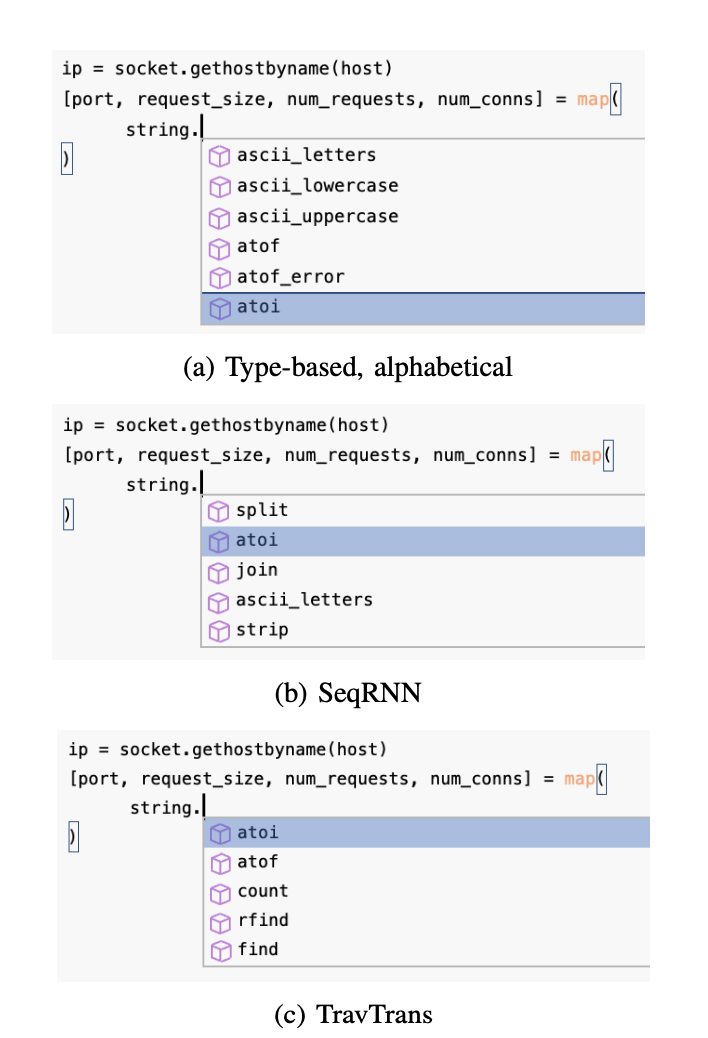
\includegraphics[width=\linewidth]{AI4CASubmissions/figs/comparison.png}
  \caption{Comparison of different next token prediction outcomes}
  \Description{Comparison of different next token prediction outcomes}
\end{figure}
\newline
\section{Limitations of existing methods and improvements}
\subsection{Limitations}
As mentioned previously, the most popular autocomplete techniques utilize popular machine learning models such as Type-based inference or sequential Recurring Neural Network (SeqRNN) ones. However, this paper points major limitations in the those two: Type-based models such as Jedi\footnote{https://github.com/davidhalter/jedi} or Eclipse\footnote{https://www.eclipse.org/pdt/help/html/working with code assist.htm} recommended and rank the next token in a very naive way (usually alphabetically), while their research has showed very clearly that popular machine learning based code prediction models such as SeqRNN recommends the next token in such a way that the correct result is present in approximately the top 2.7 results, leaving a definite margin for improvement.\cite{FeedTree}

\subsection{Improvements}
While the SeqRNN ML model yields impressive results in terms of next token recommendation, this paper's research found that using Transformer-based models for code prediction (instead of RNN) improved the ranking statistics: Correct results were displayed to developers within the first 1.5 - 2 results, an improvement of about 0.5 to 1 ranks higher.\cite{FeedTree}
\newline
A Transformer is a machine learning model first introduced by \textbf{GoogleBrain}.\footnote{https://research.google/teams/brain/} It is a type of model which processes input as a whole (for instance an entire sentence) and does not depend on past hidden states to retain past information (like Recurrent Neural Networks (RNN) do).\cite{vaswani2017attention} This has the advantage that Transformers don't risk losing past information.
\newline
An abstract syntax tree (AST) is generally defined as the abstract syntactic representation of source code.\cite{AST} Within this representation, each node of the AST represents a construct/token of the source code. The research in this paper postulates the above mentioned improvement in accuracy by feeding ASTs into Transformers. However, since Transformers are sequential models, only partial structures of the AST can be fed in at one point in time. Their solution to this was to explore three different methods to this end:\cite{FeedTree}
\begin{itemize}
    \item Decompose source code into partial programs and consequently each partial program into a sequential stream of source code tokens (SeqTrans)
    \item Decompose the AST into multiple paths and subsequently feed each path into the Transformer (PathTrans)
    \item Decompose the AST into its various traversal orders and subsequently feed each traversal into the Transformer (TravTrans)
\end{itemize}

\subsection{SeqTrans}
Since a Transformer is designed to take only sequential input, the input for this particular method works out of the box with the Transformer. A partial program (which is effectively a sequence of source code tokens) is fed as input to the Transformer, which in turn is expected to yield a single source code token as output.This method was already proven to be better than SeqRNN, as well as provided a platform for the following two AST based methods.
\subsection{PathTrans}
This method works on the concept of root paths: A root path is the path from a leaf node of an AST to to its root. Such an example is depicted in Fig 2
\begin{figure}[h]
  \centering
  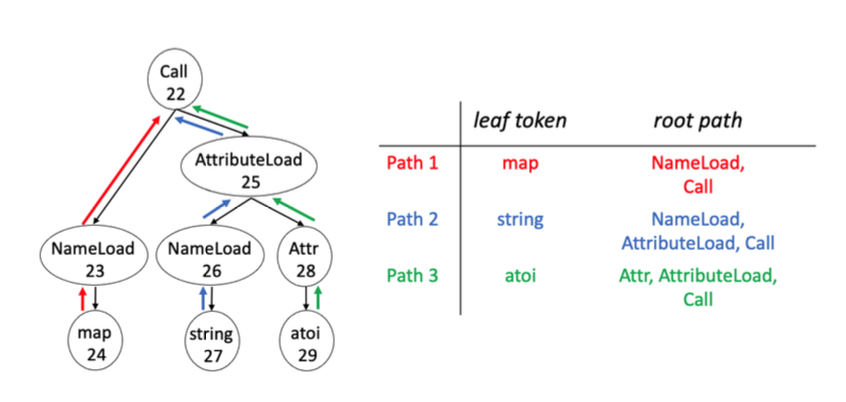
\includegraphics[width=\linewidth]{AI4CASubmissions/figs/rootpath.png}
  \caption{Rootpath concept}
  \Description{Example of leaf nodes in an AST and rootpaths to their root node}
\end{figure}
If an AST has multiple leaf nodes, there will be multiple root paths. Since each root path forms a sequence of internal nodes of the AST to each leaf token, it would ideally capture all the syntactical information along this path. Consequently, the root paths help in leaf token prediction when they are fed into the Transformer.
\subsection{TravTrans}
This method works on the concept of tree traversals;ie;feeding a sequence of nodes of the AST in a certain tree traversal order. The popular tree traversal methods include pre-order, post-order and in-order and can be applied to tree structures such as AST. The method involves feeding code token sequences which are obtained from pre-order traversals (in Depth First Search order since pre-order traversal is a kind of DFS) of the AST to optimize leaf token prediction.
\begin{figure}[h]
  \centering
  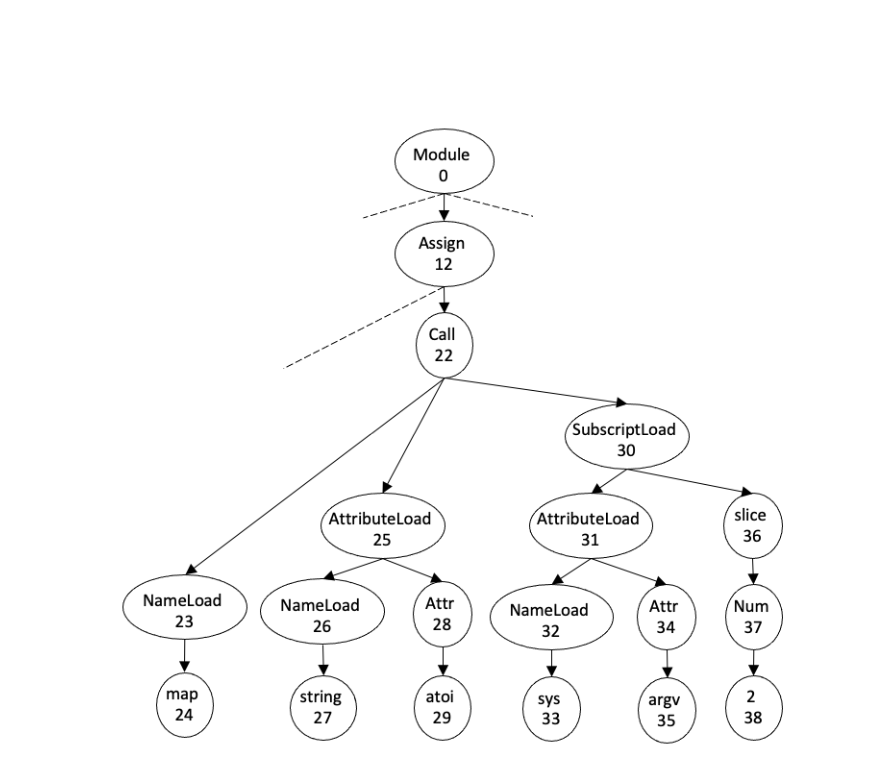
\includegraphics[width=\linewidth]{AI4CASubmissions/figs/dfs.png}
  \caption{AST as input to TravTrans}
  \Description{An AST which is decomposed is several token sequences through DFS}
\end{figure}
Fig 3 represents an AST. If we consider node 29 for example (atoi), the the node chain in DFS order preceding it would be:
\newline
\textbf{Call -> NameLoad -> Map -> AttributeLoad -> NameLoad -> string -> Attr}

\section{Implementation and Datasets}
The project mainly used two types of datasets:\cite{FeedTree}
\begin{itemize}
    \item External dataset comprising of 150k Python 2 source code files across several external GitHub repositories decomposed into ASTs. This resulted in a overall count of roughly 16 million leaf nodes.
    \item Internal dataset from GitHub repositories internal to Facebook. These also consisted of similar Python 2 source code files decomposed into ASTs. However, since the coding style was distinct, the main aim here was to ascertain consistency in prediction across disjoint projects. This also resuted in additional 1 million leaf nodes.
\end{itemize}
As for the implementation of the Transformers(SeqTrans, PathTrans and TravTrans), the project mainly used the GPT-2 small implementation\cite{radford2019language} based on the PyTorch library\footnote{https://github.com/graykode/gpt-2-Pytorch}. The schematic of a GP2 Transformer is depicted in Fig 4
\begin{figure}[h]
  \centering
  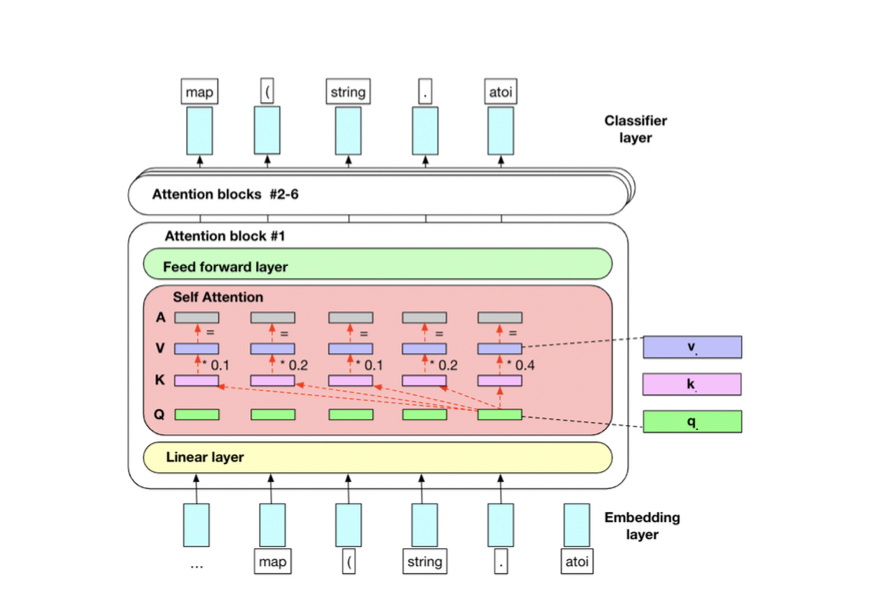
\includegraphics[width=\linewidth]{AI4CASubmissions/figs/transformer.png}
  \caption{GP2 Transformer}
  \Description{Schematic of a GP2 Transformer}
\end{figure}

\section{Result}
The token prediction results are generally expressed in terms of \textbf{mean reciprocal rank} percentages. As mentioned earlier, for typical RNN based methods, this percentage is about \textbf{37}.However, their most efficient method, \textbf{TravTrans}, which functions on feeding AST tree traversal sequences to Transformers, was found to increase this percentage by about \textbf{18}. Since 37 roughly equates to the correct token being present in the first 2.7 results, this 18 percent increase meant that now the correct token could be present anywhere between the first 1.5 and 2 results.

% References
\bibliographystyle{ACM-Reference-Format}
\bibliography{references}

%%
%% If your work has an appendix, this is the place to put it.
%\section{Appendices}
%\appendix

%\section{My Appendix}
%
%Lorem ipsum

\end{document}
\endinput
